\documentclass[]{article}
\usepackage{lmodern}
\usepackage{amssymb,amsmath}
\usepackage{ifxetex,ifluatex}
\usepackage{fixltx2e} % provides \textsubscript
\ifnum 0\ifxetex 1\fi\ifluatex 1\fi=0 % if pdftex
  \usepackage[T1]{fontenc}
  \usepackage[utf8]{inputenc}
\else % if luatex or xelatex
  \ifxetex
    \usepackage{mathspec}
  \else
    \usepackage{fontspec}
  \fi
  \defaultfontfeatures{Ligatures=TeX,Scale=MatchLowercase}
\fi
% use upquote if available, for straight quotes in verbatim environments
\IfFileExists{upquote.sty}{\usepackage{upquote}}{}
% use microtype if available
\IfFileExists{microtype.sty}{%
\usepackage{microtype}
\UseMicrotypeSet[protrusion]{basicmath} % disable protrusion for tt fonts
}{}
\usepackage[margin=1in]{geometry}
\usepackage{hyperref}
\hypersetup{unicode=true,
            pdftitle={Problem set},
            pdfauthor={Xinyi Lin},
            pdfborder={0 0 0},
            breaklinks=true}
\urlstyle{same}  % don't use monospace font for urls
\usepackage{color}
\usepackage{fancyvrb}
\newcommand{\VerbBar}{|}
\newcommand{\VERB}{\Verb[commandchars=\\\{\}]}
\DefineVerbatimEnvironment{Highlighting}{Verbatim}{commandchars=\\\{\}}
% Add ',fontsize=\small' for more characters per line
\usepackage{framed}
\definecolor{shadecolor}{RGB}{248,248,248}
\newenvironment{Shaded}{\begin{snugshade}}{\end{snugshade}}
\newcommand{\AlertTok}[1]{\textcolor[rgb]{0.94,0.16,0.16}{#1}}
\newcommand{\AnnotationTok}[1]{\textcolor[rgb]{0.56,0.35,0.01}{\textbf{\textit{#1}}}}
\newcommand{\AttributeTok}[1]{\textcolor[rgb]{0.77,0.63,0.00}{#1}}
\newcommand{\BaseNTok}[1]{\textcolor[rgb]{0.00,0.00,0.81}{#1}}
\newcommand{\BuiltInTok}[1]{#1}
\newcommand{\CharTok}[1]{\textcolor[rgb]{0.31,0.60,0.02}{#1}}
\newcommand{\CommentTok}[1]{\textcolor[rgb]{0.56,0.35,0.01}{\textit{#1}}}
\newcommand{\CommentVarTok}[1]{\textcolor[rgb]{0.56,0.35,0.01}{\textbf{\textit{#1}}}}
\newcommand{\ConstantTok}[1]{\textcolor[rgb]{0.00,0.00,0.00}{#1}}
\newcommand{\ControlFlowTok}[1]{\textcolor[rgb]{0.13,0.29,0.53}{\textbf{#1}}}
\newcommand{\DataTypeTok}[1]{\textcolor[rgb]{0.13,0.29,0.53}{#1}}
\newcommand{\DecValTok}[1]{\textcolor[rgb]{0.00,0.00,0.81}{#1}}
\newcommand{\DocumentationTok}[1]{\textcolor[rgb]{0.56,0.35,0.01}{\textbf{\textit{#1}}}}
\newcommand{\ErrorTok}[1]{\textcolor[rgb]{0.64,0.00,0.00}{\textbf{#1}}}
\newcommand{\ExtensionTok}[1]{#1}
\newcommand{\FloatTok}[1]{\textcolor[rgb]{0.00,0.00,0.81}{#1}}
\newcommand{\FunctionTok}[1]{\textcolor[rgb]{0.00,0.00,0.00}{#1}}
\newcommand{\ImportTok}[1]{#1}
\newcommand{\InformationTok}[1]{\textcolor[rgb]{0.56,0.35,0.01}{\textbf{\textit{#1}}}}
\newcommand{\KeywordTok}[1]{\textcolor[rgb]{0.13,0.29,0.53}{\textbf{#1}}}
\newcommand{\NormalTok}[1]{#1}
\newcommand{\OperatorTok}[1]{\textcolor[rgb]{0.81,0.36,0.00}{\textbf{#1}}}
\newcommand{\OtherTok}[1]{\textcolor[rgb]{0.56,0.35,0.01}{#1}}
\newcommand{\PreprocessorTok}[1]{\textcolor[rgb]{0.56,0.35,0.01}{\textit{#1}}}
\newcommand{\RegionMarkerTok}[1]{#1}
\newcommand{\SpecialCharTok}[1]{\textcolor[rgb]{0.00,0.00,0.00}{#1}}
\newcommand{\SpecialStringTok}[1]{\textcolor[rgb]{0.31,0.60,0.02}{#1}}
\newcommand{\StringTok}[1]{\textcolor[rgb]{0.31,0.60,0.02}{#1}}
\newcommand{\VariableTok}[1]{\textcolor[rgb]{0.00,0.00,0.00}{#1}}
\newcommand{\VerbatimStringTok}[1]{\textcolor[rgb]{0.31,0.60,0.02}{#1}}
\newcommand{\WarningTok}[1]{\textcolor[rgb]{0.56,0.35,0.01}{\textbf{\textit{#1}}}}
\usepackage{graphicx,grffile}
\makeatletter
\def\maxwidth{\ifdim\Gin@nat@width>\linewidth\linewidth\else\Gin@nat@width\fi}
\def\maxheight{\ifdim\Gin@nat@height>\textheight\textheight\else\Gin@nat@height\fi}
\makeatother
% Scale images if necessary, so that they will not overflow the page
% margins by default, and it is still possible to overwrite the defaults
% using explicit options in \includegraphics[width, height, ...]{}
\setkeys{Gin}{width=\maxwidth,height=\maxheight,keepaspectratio}
\IfFileExists{parskip.sty}{%
\usepackage{parskip}
}{% else
\setlength{\parindent}{0pt}
\setlength{\parskip}{6pt plus 2pt minus 1pt}
}
\setlength{\emergencystretch}{3em}  % prevent overfull lines
\providecommand{\tightlist}{%
  \setlength{\itemsep}{0pt}\setlength{\parskip}{0pt}}
\setcounter{secnumdepth}{0}
% Redefines (sub)paragraphs to behave more like sections
\ifx\paragraph\undefined\else
\let\oldparagraph\paragraph
\renewcommand{\paragraph}[1]{\oldparagraph{#1}\mbox{}}
\fi
\ifx\subparagraph\undefined\else
\let\oldsubparagraph\subparagraph
\renewcommand{\subparagraph}[1]{\oldsubparagraph{#1}\mbox{}}
\fi

%%% Use protect on footnotes to avoid problems with footnotes in titles
\let\rmarkdownfootnote\footnote%
\def\footnote{\protect\rmarkdownfootnote}

%%% Change title format to be more compact
\usepackage{titling}

% Create subtitle command for use in maketitle
\providecommand{\subtitle}[1]{
  \posttitle{
    \begin{center}\large#1\end{center}
    }
}

\setlength{\droptitle}{-2em}

  \title{Problem set}
    \pretitle{\vspace{\droptitle}\centering\huge}
  \posttitle{\par}
    \author{Xinyi Lin}
    \preauthor{\centering\large\emph}
  \postauthor{\par}
      \predate{\centering\large\emph}
  \postdate{\par}
    \date{9/25/2019}


\begin{document}
\maketitle

\hypertarget{problem-1}{%
\subsection{Problem 1}\label{problem-1}}

\hypertarget{question-a}{%
\subsubsection{Question a}\label{question-a}}

To calculate a sample size, we need additional information including:

\begin{enumerate}
\def\labelenumi{\arabic{enumi})}
\item
  The dependent variable is approximately normally distributed within
  each group.
\item
  The data is collected from a representative, randomly selected portion
  of the total population.
\item
  Sample sizes of two groups.
\end{enumerate}

\hypertarget{question-b}{%
\subsubsection{Question b}\label{question-b}}

If we assume sample size of two groups are the same and assumption 1)
and 2) are valid. As \(t = \frac{d}{var\times\sqrt{\frac{2}{n}}}\) In
order to have 5\% significance, \(t>t_{1-\frac{2}{\alpha},2n-2}\)

\begin{Shaded}
\begin{Highlighting}[]
\NormalTok{d =}\StringTok{ }\DecValTok{10}
\NormalTok{var =}\StringTok{ }\DecValTok{20}
\NormalTok{n =}\StringTok{ }\DecValTok{2}
\NormalTok{t =}\StringTok{ }\NormalTok{d}\OperatorTok{/}\NormalTok{(var}\OperatorTok{*}\KeywordTok{sqrt}\NormalTok{(}\DecValTok{2}\OperatorTok{/}\NormalTok{n))}
\ControlFlowTok{while}\NormalTok{ (t}\OperatorTok{<=}\KeywordTok{qt}\NormalTok{(}\FloatTok{0.975}\NormalTok{, }\DecValTok{2}\OperatorTok{*}\NormalTok{n}\DecValTok{-2}\NormalTok{)) \{}
\NormalTok{  n =}\StringTok{ }\NormalTok{n}\OperatorTok{+}\DecValTok{1}
\NormalTok{  t =}\StringTok{ }\NormalTok{d}\OperatorTok{/}\NormalTok{(var}\OperatorTok{*}\KeywordTok{sqrt}\NormalTok{(}\DecValTok{2}\OperatorTok{/}\NormalTok{n))}
\NormalTok{\}}
\NormalTok{n}
\end{Highlighting}
\end{Shaded}

\begin{verbatim}
## [1] 32
\end{verbatim}

The sample size is 32.

\hypertarget{problem-2}{%
\subsection{Problem 2}\label{problem-2}}

\hypertarget{question-a-1}{%
\subsubsection{Question a}\label{question-a-1}}

\begin{Shaded}
\begin{Highlighting}[]
\DecValTok{14}\OperatorTok{*}\KeywordTok{pbinom}\NormalTok{(}\DecValTok{0}\NormalTok{, }\DecValTok{14}\NormalTok{, }\FloatTok{0.05}\NormalTok{) }\OperatorTok{+}\StringTok{ }\DecValTok{34}\OperatorTok{*}\NormalTok{(}\DecValTok{1}\OperatorTok{-}\KeywordTok{pbinom}\NormalTok{(}\DecValTok{0}\NormalTok{, }\DecValTok{14}\NormalTok{, }\FloatTok{0.05}\NormalTok{))}
\end{Highlighting}
\end{Shaded}

\begin{verbatim}
## [1] 24.2465
\end{verbatim}

The expected value of the sample size is around 24.25.

\hypertarget{question-b-1}{%
\subsubsection{Question b}\label{question-b-1}}

Let \(R_i\) be the number of responses in the first or second stages,
where \(i \in\{1,2\}\).

The probability of a ``go'' decision is \[\begin{split}
P_b&=\sum_{j=1}^4[P(R_1+R_2\geq4)]+P(R_1>4) \\
&=\sum_{j=1}^4[P(R_2>3-j,R_1=j)]+P(R_1>4) \\
&=\sum_{j=1}^4[P(R_2>3-j)P(R_1=j)]+P(R_1>4)
\end{split}\].

\begin{Shaded}
\begin{Highlighting}[]
\KeywordTok{pbinom}\NormalTok{(}\DecValTok{2}\NormalTok{, }\DecValTok{20}\NormalTok{, }\FloatTok{0.05}\NormalTok{, }\DataTypeTok{lower.tail =} \OtherTok{FALSE}\NormalTok{)}\OperatorTok{*}\KeywordTok{dbinom}\NormalTok{(}\DecValTok{1}\NormalTok{, }\DecValTok{14}\NormalTok{, }\FloatTok{0.05}\NormalTok{) }\OperatorTok{+}\StringTok{ }\KeywordTok{pbinom}\NormalTok{(}\DecValTok{1}\NormalTok{, }\DecValTok{20}\NormalTok{, }\FloatTok{0.05}\NormalTok{, }\DataTypeTok{lower.tail =} \OtherTok{FALSE}\NormalTok{)}\OperatorTok{*}\KeywordTok{dbinom}\NormalTok{(}\DecValTok{2}\NormalTok{, }\DecValTok{14}\NormalTok{, }\FloatTok{0.05}\NormalTok{) }\OperatorTok{+}\StringTok{ }\KeywordTok{pbinom}\NormalTok{(}\DecValTok{0}\NormalTok{, }\DecValTok{20}\NormalTok{, }\FloatTok{0.05}\NormalTok{, }\DataTypeTok{lower.tail =} \OtherTok{FALSE}\NormalTok{)}\OperatorTok{*}\KeywordTok{dbinom}\NormalTok{(}\DecValTok{3}\NormalTok{, }\DecValTok{14}\NormalTok{, }\FloatTok{0.05}\NormalTok{) }\OperatorTok{+}\StringTok{ }\KeywordTok{pbinom}\NormalTok{(}\DecValTok{3}\NormalTok{, }\DecValTok{14}\NormalTok{, }\FloatTok{0.05}\NormalTok{, }\DataTypeTok{lower.tail =} \OtherTok{FALSE}\NormalTok{)}
\end{Highlighting}
\end{Shaded}

\begin{verbatim}
## [1] 0.0803739
\end{verbatim}

So the probability of a ``go'' decision is around 0.080.

\hypertarget{question-c}{%
\subsubsection{Question c}\label{question-c}}

\begin{Shaded}
\begin{Highlighting}[]
\KeywordTok{pbinom}\NormalTok{(}\DecValTok{2}\NormalTok{, }\DecValTok{20}\NormalTok{, }\FloatTok{0.2}\NormalTok{, }\DataTypeTok{lower.tail =} \OtherTok{FALSE}\NormalTok{)}\OperatorTok{*}\KeywordTok{dbinom}\NormalTok{(}\DecValTok{1}\NormalTok{, }\DecValTok{14}\NormalTok{, }\FloatTok{0.2}\NormalTok{) }\OperatorTok{+}\StringTok{ }\KeywordTok{pbinom}\NormalTok{(}\DecValTok{1}\NormalTok{, }\DecValTok{20}\NormalTok{, }\FloatTok{0.2}\NormalTok{, }\DataTypeTok{lower.tail =} \OtherTok{FALSE}\NormalTok{)}\OperatorTok{*}\KeywordTok{dbinom}\NormalTok{(}\DecValTok{2}\NormalTok{, }\DecValTok{14}\NormalTok{, }\FloatTok{0.2}\NormalTok{) }\OperatorTok{+}\StringTok{ }\KeywordTok{pbinom}\NormalTok{(}\DecValTok{0}\NormalTok{, }\DecValTok{20}\NormalTok{, }\FloatTok{0.2}\NormalTok{, }\DataTypeTok{lower.tail =} \OtherTok{FALSE}\NormalTok{)}\OperatorTok{*}\KeywordTok{dbinom}\NormalTok{(}\DecValTok{3}\NormalTok{, }\DecValTok{14}\NormalTok{, }\FloatTok{0.2}\NormalTok{) }\OperatorTok{+}\StringTok{ }\KeywordTok{pbinom}\NormalTok{(}\DecValTok{3}\NormalTok{, }\DecValTok{14}\NormalTok{, }\FloatTok{0.2}\NormalTok{, }\DataTypeTok{lower.tail =} \OtherTok{FALSE}\NormalTok{)}
\end{Highlighting}
\end{Shaded}

\begin{verbatim}
## [1] 0.9041092
\end{verbatim}

When the true response rate is 20\%, the probability of a ``go''
decision is around 0.904.

\hypertarget{question-d}{%
\subsubsection{Question d}\label{question-d}}

Let \(n\) be the sample size of the fixed design, \(R\) be the number of
response in the trial, if there is at least \(x\) response, then the
treatment is deemed promising (``go'')

\[type \ I \ error = P(reject \ null|null \ is \ true) = P(R>X|p=0.05)\]
\[power = P(reject \ null|alternative \ is \ true) = P(R>X|p=0.2)\]

\begin{Shaded}
\begin{Highlighting}[]
\NormalTok{n =}\StringTok{ }\DecValTok{3}
\NormalTok{x =}\StringTok{ }\DecValTok{1}
\ControlFlowTok{while}\NormalTok{(}\KeywordTok{pbinom}\NormalTok{(x}\DecValTok{-1}\NormalTok{,n,}\FloatTok{0.05}\NormalTok{,}\DataTypeTok{lower.tail =} \OtherTok{FALSE}\NormalTok{)}\OperatorTok{>}\FloatTok{0.080} \OperatorTok{|}\StringTok{ }\KeywordTok{pbinom}\NormalTok{(x}\DecValTok{-1}\NormalTok{,n,}\FloatTok{0.2}\NormalTok{,}\DataTypeTok{lower.tail =} \OtherTok{FALSE}\NormalTok{)}\OperatorTok{<}\FloatTok{0.904}\NormalTok{)\{}
  \ControlFlowTok{if}\NormalTok{(x}\OperatorTok{<}\NormalTok{n}\DecValTok{-1}\NormalTok{)\{}
\NormalTok{    x =}\StringTok{ }\NormalTok{x}\OperatorTok{+}\DecValTok{1}
\NormalTok{  \} }\ControlFlowTok{else}\NormalTok{ \{}
\NormalTok{    x =}\StringTok{ }\DecValTok{1}
\NormalTok{    n =}\StringTok{ }\NormalTok{n}\OperatorTok{+}\DecValTok{1}\NormalTok{\}}
\NormalTok{\}}
\NormalTok{n}
\end{Highlighting}
\end{Shaded}

\begin{verbatim}
## [1] 32
\end{verbatim}

The sample size required for a fixed design with null response 5\% and
alternative response 20\% is 32.

\hypertarget{problem-3}{%
\subsection{Problem 3}\label{problem-3}}

\hypertarget{question-a-2}{%
\subsubsection{Question a}\label{question-a-2}}

Assume,
\(\lambda\sim\Gamma(\alpha,\beta), f(\lambda|\alpha,\beta) = \frac{\beta^{\alpha}\lambda^{\alpha-1}e^{-\beta\lambda}}{\Gamma(\alpha)}\),
for \(\lambda>0\).

\[\begin{split}
f(x)&=\int_0^{+\infty}f(x|\lambda)f(\lambda)d\lambda\\
&=\int_0^{+\infty}\lambda e^{-\lambda x}\frac{\beta^\alpha\lambda^{\alpha-1}e^{-\beta\lambda}}{\Gamma(\alpha)}d\lambda\\
&=\int_0^{+\infty}\frac{\lambda^\alpha\beta^\alpha e^{-(\beta+x)\lambda}}{\Gamma(\alpha)}d\lambda\\
&=\int_0^{+\infty}\frac{\lambda^{(\alpha+1)-1}(\beta+x)^{\alpha+1}e^{-(\beta+x)\lambda}}{\Gamma(\alpha+1)}\frac{\beta^\alpha(\alpha+1)}{(\beta+x)^{\alpha+1}}d\lambda\\
&=\frac{\beta^\alpha(\alpha+1)}{(\beta+x)^{\alpha+1}}
\end{split}\]

Posterior Distribution:

\[\begin{split}
f(\lambda|x)&=\frac{f(x_1|\lambda)f(\lambda)}{f(x_1)}\\
&=\frac{\lambda e^{-\lambda x_1}\frac{\beta^\alpha \lambda^{\alpha-1}e^{-\beta\lambda}}{\Gamma(\alpha)}}{\frac{\beta^\alpha(\alpha+1)}{(\beta+x_1)^{\alpha+1}}}\\
&=\frac{\lambda e^{-\lambda x_1}\lambda^{\alpha-1}e^{-\beta\lambda}(\beta+x_1)^{\alpha+1}}{\Gamma(\alpha+1)}\\
&=\frac{e^{-\lambda(x_1+\beta)}\lambda^\alpha(\beta+x_1)^{\alpha+1}}{\Gamma(\alpha+1)}\\
&=\Gamma(\alpha+1,\beta+x)
\end{split}\]

\hypertarget{question-b-2}{%
\subsubsection{Question b}\label{question-b-2}}

\[\begin{split}
f(x_2|x_1)&=\frac{f(x_1,x_2)}{f(x_1)}=\frac{\int_0^{+\infty}f(x_1|\lambda)f(x_2|\lambda)f(\lambda)d\lambda}{f(x_1)}\\
&=\frac{\int_0^{+\infty}\lambda e^{-\lambda x_1}\lambda e^{-\lambda x_2}\frac{\beta^\alpha\lambda^{\alpha-1}e^{-\beta\lambda}}{\Gamma(\alpha)}d\lambda}{\frac{\beta^\alpha(\alpha+1)}{(\beta+x_1)^{\alpha+1}}}\\
&=\int_0^{+\infty}\frac{\lambda^{\alpha+1}e^{-\lambda(x_1+x_2+\beta)}(\beta+x_1)^{\alpha+1}}{\Gamma(\alpha+1)}d\lambda\\
&=\int_0^{+\infty}\frac{\lambda^{\alpha+1}e^{-\lambda(x_1+x_2+\beta)}(\beta+x_1+x_2)^{\alpha+2}}{\Gamma(\alpha+2)}\frac{(\beta+x_1)^{\alpha+1}(\alpha+2)}{(\beta+x_1+x_2)^{\alpha+2}}d\lambda\\
&=\frac{(\beta+x_1)^{\alpha+1}(\alpha+2)}{(\beta+x_1+x_2)^{\alpha+2}}
\end{split}\]

\hypertarget{question-c-1}{%
\subsubsection{Question c}\label{question-c-1}}

\[\left\{
\begin{aligned}
Y_1 & = \frac{X_1+X_2}{2} \\
Y_2 & = X_1 \\
\end{aligned}
\right.\]

\[J = \left| \begin{array} {cc}
\frac{\partial Y_1}{\partial X_1} & \frac{\partial Y_1}{\partial X_2}\\
\frac{\partial Y_2}{\partial X_1} & \frac{\partial Y_2}{\partial X_2}\\
\end{array} \right | =
\left| \begin{array} {cc}
1/2 & 1/2\\
1 & 0\\
\end{array} \right | = -1/2\]

\[\begin{split}
f(\frac{x_1+x_2}{2}|x_1)&= \frac{f(\frac{x_1+x_2}{2},x_1)}{f(x_1)}=\frac{f(y_1,y_2)}{f(x_1)} = -\frac{f(x_1,x_2)}{2f(x_1)}\\
&= -\frac{(\beta+x_1)^{\alpha+1}(\alpha+2)}{2(\beta+x_1+x_2)^{\alpha+2}}
\end{split}\]

\hypertarget{problem-4}{%
\subsection{Problem 4}\label{problem-4}}

Dose level 1 is safe:

1.number of DLT equals to 0 or

2.number of DLT equals to 1 and numbers of DLT equals to 0 for another 3
patients at same level.

\begin{Shaded}
\begin{Highlighting}[]
\KeywordTok{dbinom}\NormalTok{(}\DecValTok{0}\NormalTok{,}\DecValTok{3}\NormalTok{,}\FloatTok{0.25}\NormalTok{)}\OperatorTok{+}\KeywordTok{dbinom}\NormalTok{(}\DecValTok{1}\NormalTok{,}\DecValTok{3}\NormalTok{,}\FloatTok{0.25}\NormalTok{)}\OperatorTok{*}\KeywordTok{dbinom}\NormalTok{(}\DecValTok{0}\NormalTok{,}\DecValTok{3}\NormalTok{,}\FloatTok{0.25}\NormalTok{)}
\end{Highlighting}
\end{Shaded}

\begin{verbatim}
## [1] 0.5998535
\end{verbatim}

The probaility that the 3+3 algorithm declare dose level 1 is safe is
0.600.

\hypertarget{problem-5}{%
\subsection{Problem 5}\label{problem-5}}

\hypertarget{question-a-3}{%
\subsubsection{Question a}\label{question-a-3}}

Dose 1: 0.007 0.135 0.772 \textless{} 0.02 1/3 \textbar{} 0.444 0.287
0.347 \textless{} 0.02 0/3

Dose 2: 0.777 0.604 0.025 \textless{} 0.04 1/3 \textbar{} 0.584 0.715
0.110 \textless{} 0.04 0/3

Dose 3: 0.770 0.405 0.742 \textless{} 0.1 0/3

Dose 4: 0.923 0.591 0.567 \textless{} 0.25 0/3

Dose 5: 0.952 0.039 0.342 \textless{} 0.5 2/3

MTD = 4

\hypertarget{question-b-3}{%
\subsubsection{Question b}\label{question-b-3}}

\begin{itemize}
\tightlist
\item
  Trial 1
\end{itemize}

Dose 1: 0.534 0.342 0.661 \textless{} 0.02 0/3

Dose 2: 0.829 0.489 0.710 \textless{} 0.04 0/3

Dose 3: 0.921 0.055 0.497 \textless{} 0.1 1/3 \textbar{} 0.611 0.118
0.122 \textless{} 0.1 0/3

Dose 4: 0.472 0.853 0.931 \textless{} 0.25 0/3

Dose 5: 0.978 0.232 0.519 \textless{} 0.5 1/3 \textbar{} 0.333 0.096
0.709 \textless{} 0.5 2/3

MTD = 4

\begin{itemize}
\tightlist
\item
  Trial 2
\end{itemize}

Dose 1: 0.985 0.844 0.948 \textless{} 0.02 0/3

Dose 2: 0.361 0.061 0.541 \textless{} 0.04 0/3

Dose 3: 0.815 0.153 0.177 \textless{} 0.1 0/3

Dose 4: 0.495 0.735 0.872 \textless{} 0.25 0/3

Dose 5: 0.799 0.028 0.555 \textless{} 0.5 1/3 \textbar{} 0.763 0.752
0.682 \textless{} 0.5 0/3

MTD = 5

\begin{itemize}
\tightlist
\item
  Trial 3
\end{itemize}

Dose 1: 0.228 0.586 0.732 \textless{} 0.01 0/3

Dose 2: 0.014 0.753 0.412 \textless{} 0.04 1/3 \textbar{} 0.765 0.176
0.919 \textless{} 0.04 0/3

Dose 3: 0.207 0.874 0.178 \textless{} 0.1 0/3

Dose 4: 0.820 0.783 0.231 \textless{} 0.25 1/3 \textbar{} 0.541 0.925
0.207 \textless{} 0.25 1/3

MTD = 3

\begin{itemize}
\tightlist
\item
  Trial 4
\end{itemize}

Dose 1: 0.408 0.808 0.434 \textless{} 0.02 0/3

Does 2: 0.008 0.382 0.166 \textless{} 0.04 1/3 \textbar{} 0.328 0.294
0.635 \textless{} 0.04 0/3

Dose 3: 0.672 0.669 0.460 \textless{} 0.1 0/3

Dose 4: 0.174 0.374 0.381 \textless{} 0.25 1/3 \textbar{} 0.600 0.397
0.091 \textless{} 0.25 1/3

MTD = 3

\begin{itemize}
\tightlist
\item
  Trial 5
\end{itemize}

Dose 1: 0.922 0.872 0.754 \textless{} 0.02 0/3

Dose 2: 0.520 0.977 0.748 \textless0.04 0/3

Dose 3: 0.955 0.978 0.531 \textless{} 0.1 0/3

Dose 4: 0.196 0.963 0.356 \textless0.25 1/3 \textbar{} 0.061 0.795 0.823
\textless{} 0.25 1/3

MTD = 3

\begin{itemize}
\tightlist
\item
  Trial 6
\end{itemize}

Dose 1: 0.731 0.284 0.929 \textless0.02 0/3

Dose 2: 0.687 0.858 0.439 \textless0.04 0/3

Dose 3: 0.944 0.676 0.189 \textless{} 0.1 0/3

Dose 4: 0.755 0.421 0.357 \textless0.25 0/3

Dose 5: 0.391 0.370 0.028 \textless0.5 3/3

MTD = 4

\begin{itemize}
\tightlist
\item
  Trial 7
\end{itemize}

Dose 1: 0.866 0.069 0.818 \textless{} 0.02 0/3

Dose 2: 0.888 0.381 0.989 \textless{} 0.04 0/3

Dose 3: 0.663 0.491 0.285 \textless{} 0.1 0/3

Dose 4: 0.000 0.652 0.341 \textless{} 0.25 1/3 \textbar{} 0.316 0.599
0.977 \textless{} 0.25 0/3

Dose 5: 0.332 0.985 0.976 \textless{} 0.5 1/3 \textbar{} 0.695 0.730
0.580 \textless{} 0.5 0/3

MTD = 5

\begin{itemize}
\tightlist
\item
  Trial 8
\end{itemize}

Dose 1: 0.562 0.674 0.435 \textless{} 0.02 0/3

Dose 2: 0.747 0.521 0.024 \textless{} 0.04 1/3 \textbar{} 0.412 0.719
0.819 \textless0.04 0/3

Dose 3: 0.139 0.278 0.270 \textless{} 0.1 0/3

Dose 4: 0.877 0.431 0.867 \textless{} 0.25 0/3

Dose 5: 0.723 0.919 0.244 \textless0.5 1/3 \textbar{} 0.362 0.442 0.196
\textless0.5 3/3

MTD = 4

\begin{itemize}
\tightlist
\item
  Trial 9
\end{itemize}

Dose 1: 0.409 0.752 0.351 \textless0.02 0/3

Dose 2: 0.979 0.189 0.523 \textless0.04 0/3

Dose 3: 0.332 0.690 0.061 \textless0.1 1/3 \textbar{} 0.552 0.253 0.450
\textless0.1 0/3

Dose 4: 0.403 0.592 0.381 \textless0.25 0/3

Dose 5:

0.673 0.182 0.862 \textless0.5 1/3 \textbar{} 0.223 0.090 0.729
\textless0.5 2/3

MTD = 4

\begin{itemize}
\tightlist
\item
  Trial 10
\end{itemize}

Dose 1 0.091 0.315 0.763 \textless0.02 0/3

Dose 2 0.373 0.174 0.927 \textless{} 0.04 0/3

Dose 3 0.264 0.799 0.653 \textless0.1 0/3

Dose 4 0.569 0.109 0.706 \textless0.25 1/3 \textbar{} 0.858 0.357 0.950
\textless0.25 0/3

Dose 5 0.801 0.123 0.019 \textless0.5 2/3

MTD = 4

\begin{Shaded}
\begin{Highlighting}[]
\KeywordTok{data.frame}\NormalTok{(}\DataTypeTok{Dose =} \DecValTok{0}\OperatorTok{:}\DecValTok{5}\NormalTok{, }\DataTypeTok{probability =} \KeywordTok{c}\NormalTok{(}\DecValTok{0}\NormalTok{,}\DecValTok{0}\NormalTok{,}\DecValTok{0}\NormalTok{,}\DecValTok{3}\NormalTok{,}\DecValTok{5}\NormalTok{,}\DecValTok{2}\NormalTok{)}\OperatorTok{/}\DecValTok{10}\NormalTok{)}
\end{Highlighting}
\end{Shaded}

\begin{verbatim}
##   Dose probability
## 1    0         0.0
## 2    1         0.0
## 3    2         0.0
## 4    3         0.3
## 5    4         0.5
## 6    5         0.2
\end{verbatim}

\hypertarget{problem-6}{%
\subsection{Problem 6}\label{problem-6}}

\begin{Shaded}
\begin{Highlighting}[]
\KeywordTok{library}\NormalTok{(dfcrm)}
\NormalTok{target =}\StringTok{ }\FloatTok{0.1}
\NormalTok{prior =}\StringTok{ }\KeywordTok{c}\NormalTok{(}\FloatTok{0.05}\NormalTok{, }\FloatTok{0.12}\NormalTok{, }\FloatTok{0.25}\NormalTok{, }\FloatTok{0.40}\NormalTok{, }\FloatTok{0.55}\NormalTok{)}
\NormalTok{trueP =}\StringTok{ }\KeywordTok{c}\NormalTok{(}\FloatTok{0.02}\NormalTok{, }\FloatTok{0.04}\NormalTok{, }\FloatTok{0.10}\NormalTok{, }\FloatTok{0.25}\NormalTok{, }\FloatTok{0.50}\NormalTok{)}
\NormalTok{N =}\StringTok{ }\DecValTok{20}
\NormalTok{crmoutput =}\StringTok{ }\KeywordTok{crmsim}\NormalTok{(trueP, prior, target, N, }\DecValTok{3}\NormalTok{, }\DataTypeTok{model =} \StringTok{"logistic"}\NormalTok{)}
\NormalTok{crmoutput}\OperatorTok{$}\NormalTok{MTD}
\end{Highlighting}
\end{Shaded}

\begin{verbatim}
## [1] 2
\end{verbatim}

\hypertarget{problem-7}{%
\subsection{Problem 7}\label{problem-7}}

\begin{Shaded}
\begin{Highlighting}[]
\NormalTok{crmoutput =}\StringTok{ }\KeywordTok{crmsim}\NormalTok{(trueP, prior, target, N, }\DecValTok{3}\NormalTok{, }\DataTypeTok{nsim =} \DecValTok{10}\NormalTok{, }\DataTypeTok{model =} \StringTok{"logistic"}\NormalTok{)}
\end{Highlighting}
\end{Shaded}

\begin{verbatim}
## simulation number: 1 
## simulation number: 2 
## simulation number: 3 
## simulation number: 4 
## simulation number: 5 
## simulation number: 6 
## simulation number: 7 
## simulation number: 8 
## simulation number: 9 
## simulation number: 10
\end{verbatim}

\begin{Shaded}
\begin{Highlighting}[]
\KeywordTok{data.frame}\NormalTok{(}\DataTypeTok{dose =}\NormalTok{ 1:5, }\DataTypeTok{probability =}\NormalTok{ crmoutput}\OperatorTok{$}\NormalTok{MTD)}
\end{Highlighting}
\end{Shaded}

\begin{verbatim}
##   dose probability
## 1    1         0.0
## 2    2         0.1
## 3    3         0.6
## 4    4         0.3
## 5    5         0.0
\end{verbatim}

\hypertarget{problem-8}{%
\subsection{Problem 8}\label{problem-8}}

Assume \(\lambda_1 \sim \Gamma(\alpha_1,\beta_1)\),
\(\lambda_2 \sim \Gamma(\alpha_2,\beta_2)\)

\[Pr(\lambda_1>\lambda_2|x_1,...,x_n,y_1,...,y_m)=Pr((\lambda_1|x_1,...,x_n)>(\lambda_2|y_1,...,y_m))\]
where
\[\lambda_1|x_1,...,x_n \sim \Gamma(\alpha_1+n, \beta_1+\sum_{i=1}^nx_i), \lambda_2|y_1,...,y_m~\Gamma(\alpha_2+m,\beta_2+\sum_{j=1}^my_j)\]

Given
\(\alpha_1, \alpha_2, \beta_1, \beta_2, n, m, \sum_{i=1}^nx_i, \sum_{j=1}^my_j\),
we can simulate 1000 \(\lambda_1\) and \(\lambda_2\) and calculate
\(Pr(\lambda_1>\lambda_2|x_1,...,x_n,y_1,...,y_m)\).

\(Pr(\lambda_1>\lambda_2|x_1,...,x_n,y_1,...,y_m)=\int_0^\infty\int_0^{\lambda_1}\Gamma(\alpha_1+n, \beta_1+\sum_{i=1}^nx_i)\Gamma(\alpha_2+m,\beta_2+\sum_{j=1}^my_j)d\lambda_2d\lambda_1\)

\hypertarget{problem-9}{%
\subsection{Problem 9}\label{problem-9}}

\hypertarget{question-a-4}{%
\subsubsection{Question a}\label{question-a-4}}

\begin{figure}
\centering
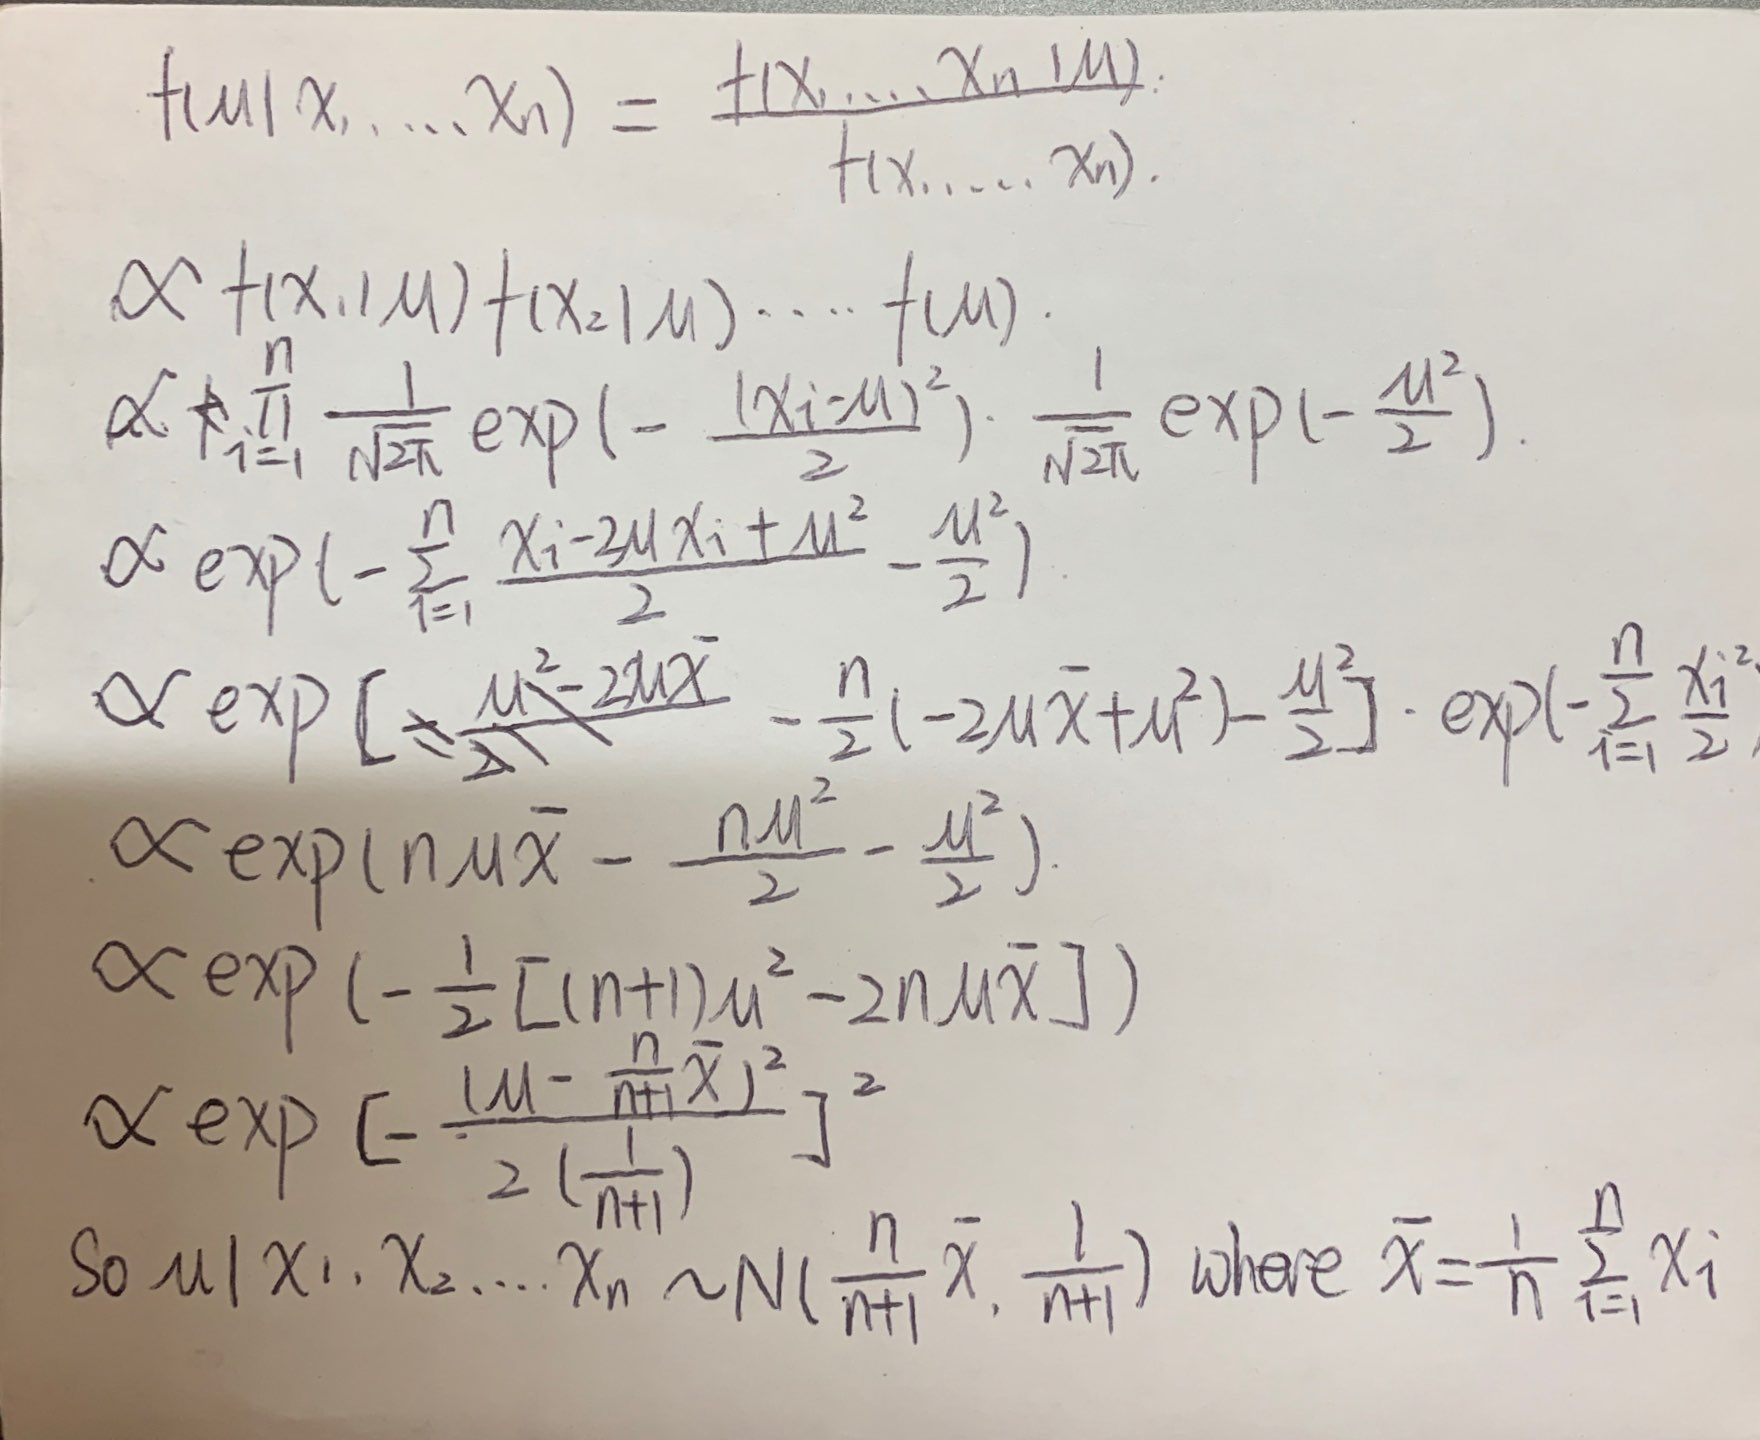
\includegraphics{./Problem9.jpg}
\caption{Problem 9 Question a.}
\end{figure}

\hypertarget{question-b-4}{%
\subsubsection{Question b}\label{question-b-4}}

According to Question a,
\(v|y_1,...,y_m \sim N(\frac{m}{m+1}\bar y,\frac{1}{m+1})\) where
\(\bar y = \frac{1}{n}\sum_{i=1}^ny_i\)

As \(x_i\) and \(y_i\) are independent

\(Pr(\mu>v|x_1, ...,x_n, y_1, ...,y_m)=\int_{-\infty}^{+\infty}\int_{-\infty}^\mu f(\mu,v|x_1, ...,x_n, y_1, ...,y_m)=\int_{-\infty}^{+\infty}\int_{-\infty}^\mu f(\mu|x_1,...,x_m)f(v|y_1,...,y_m)=\int_{-\infty}^{+\infty}\int_{-\infty}^\mu\frac{1}{\sqrt{\frac{4\pi^2}{(n+1)(m+1)}}}exp(-\frac{(\mu-\frac{n}{n+1}\bar x)^2}{\frac{2}{n+1}}-\frac{v-\frac{m}{m+1}\bar y)^2}{\frac{2}{m+1}})dvd\mu\)

\hypertarget{problem-10}{%
\subsection{Problem 10}\label{problem-10}}

\hypertarget{question-a-5}{%
\subsubsection{Question a}\label{question-a-5}}

\[L(\alpha,\beta,\sigma^2|x_i,y_i,i = 1,2,...,n)=\prod_{i=1}^n\frac{1}{\sqrt{2\pi\sigma^2}}e^{-\frac{(y_i-(\alpha+\beta x_i))^2}{2\sigma^2}}\]

\[l(\alpha,\beta,\sigma^2|x_i,y_i,i = 1,2,...,n)=-\frac{n}{2}log(2\pi)-nlog\sigma-\frac{1}{2\sigma^2}\sum_{i=1}^n(y_i-(\alpha+\beta x_i))^2\]

\[\hat\beta=\frac{\sum_{i=1}^n(x_i-\bar x)(y_i-\bar y)}{\sum_{i=1}^n(x_i-\bar x)^2}\]

\[\hat\alpha=\bar y-\hat\beta\bar x\]

\[\hat\sigma^2=\frac{1}{n}\sum_{i=1}^n(y_i-(\hat\alpha+\hat\beta x_i))^2\]

\begin{figure}
\centering
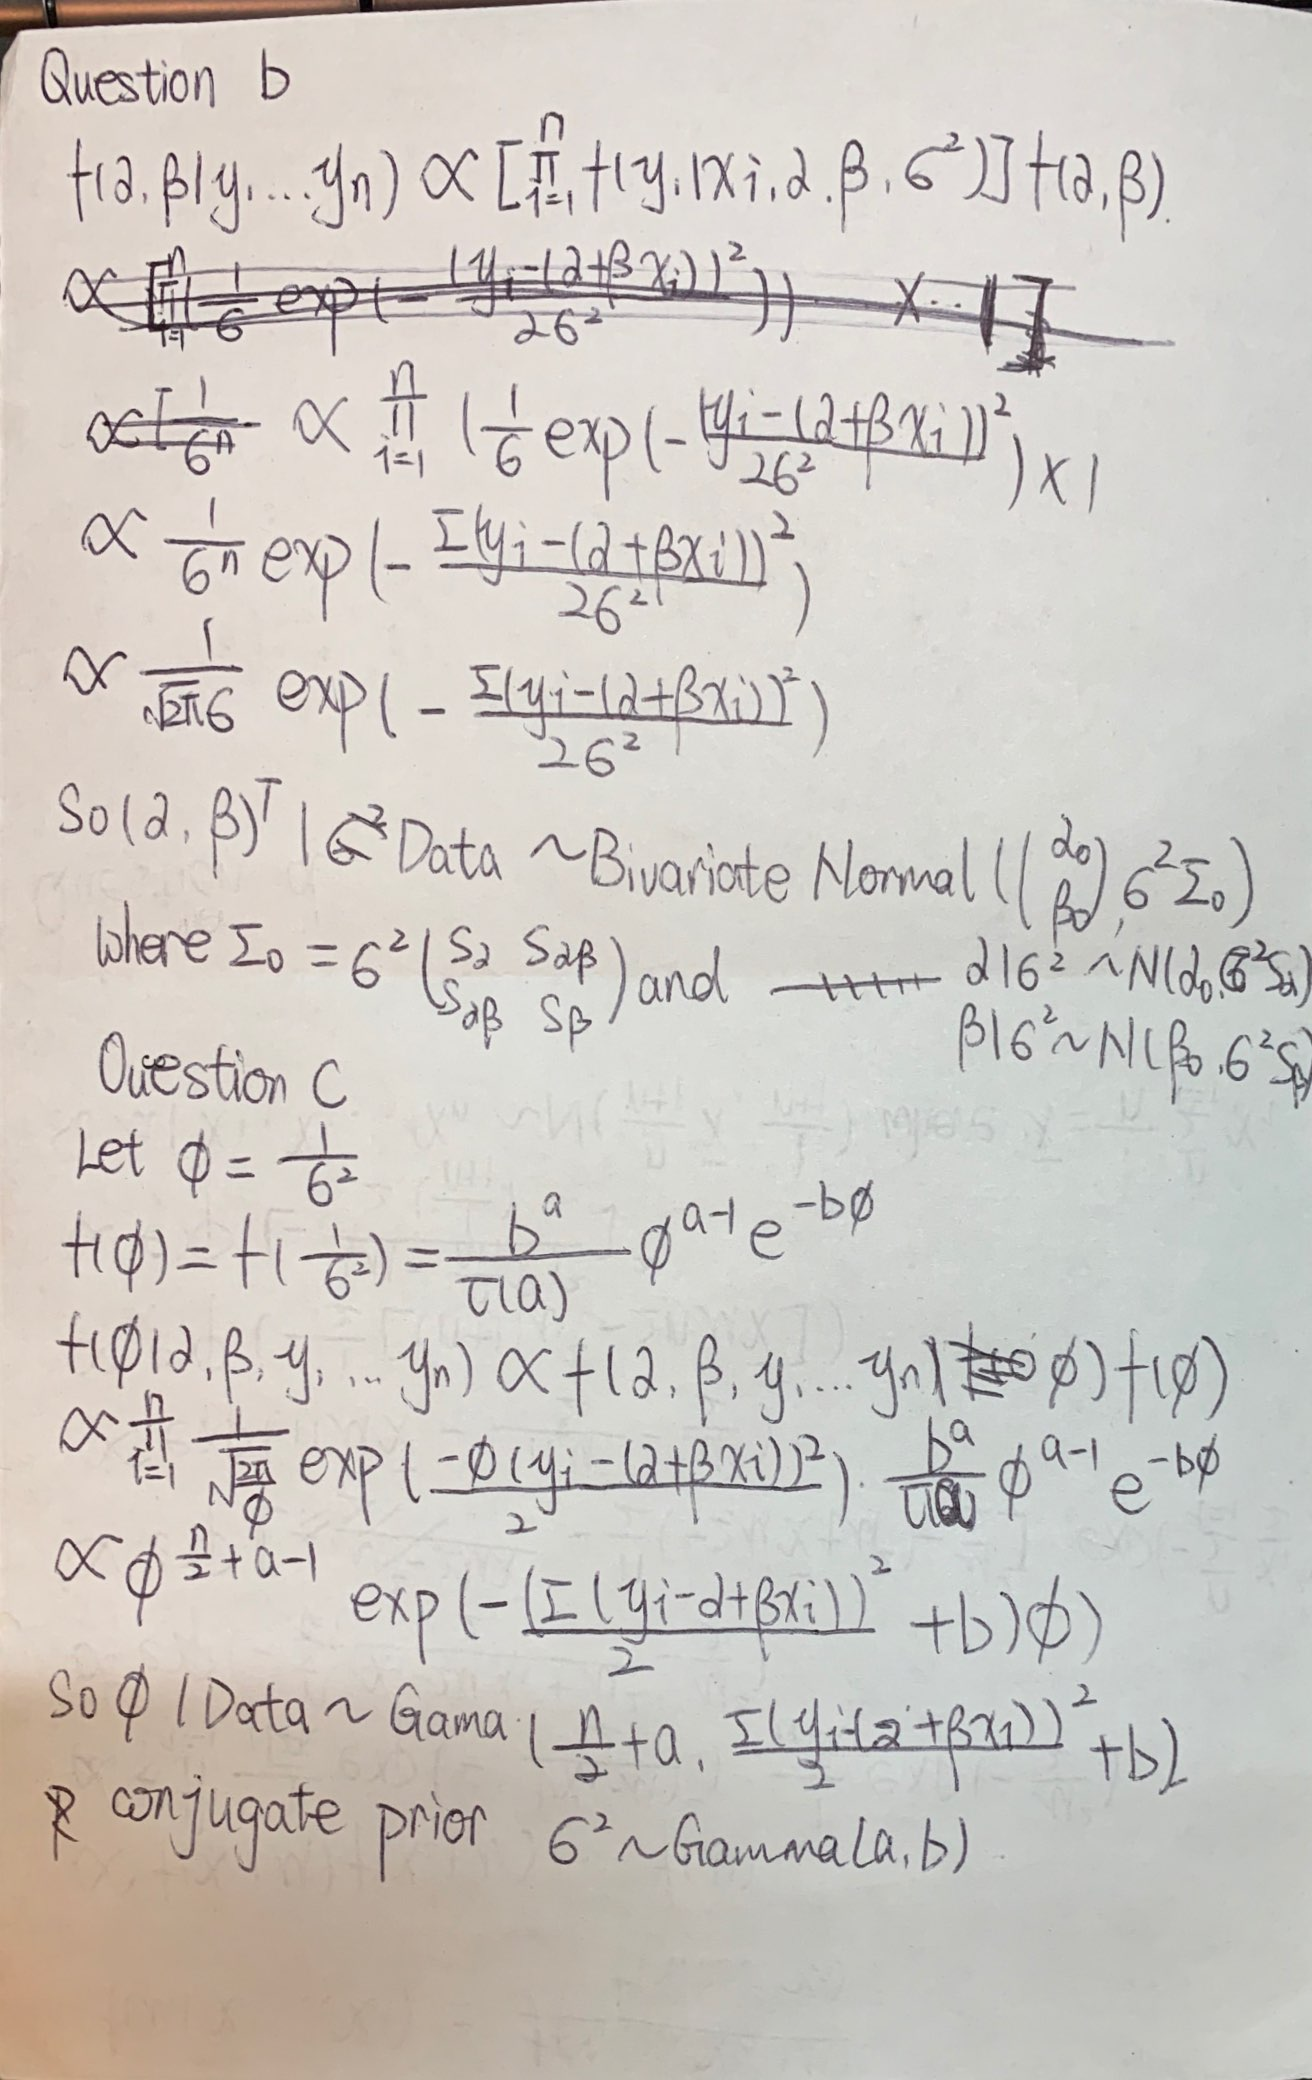
\includegraphics{./Problem10.jpg}
\caption{Problem 10 Question b\&c.}
\end{figure}

\hypertarget{problem-11}{%
\subsection{Problem 11}\label{problem-11}}

\hypertarget{question-a-6}{%
\subsubsection{Question a}\label{question-a-6}}

\begin{Shaded}
\begin{Highlighting}[]
\NormalTok{assign_Trt =}\StringTok{ }\ControlFlowTok{function}\NormalTok{(}\DataTypeTok{pA =} \FloatTok{0.2}\NormalTok{, }\DataTypeTok{pB =} \FloatTok{0.8}\NormalTok{) \{}
\NormalTok{  Treatment =}\StringTok{ }\KeywordTok{rep}\NormalTok{(}\OtherTok{NA}\NormalTok{,}\DecValTok{4}\NormalTok{)}
\NormalTok{  Treatment[}\DecValTok{1}\NormalTok{] =}\StringTok{ }\KeywordTok{rbinom}\NormalTok{(}\DecValTok{1}\NormalTok{,}\DecValTok{1}\NormalTok{,}\FloatTok{0.5}\NormalTok{) }\CommentTok{# 0 for A, 1 for B}
  \ControlFlowTok{for}\NormalTok{ (i }\ControlFlowTok{in} \DecValTok{2}\OperatorTok{:}\DecValTok{4}\NormalTok{) \{}
    \ControlFlowTok{if}\NormalTok{(Treatment[i}\DecValTok{-1}\NormalTok{]}\OperatorTok{==}\DecValTok{0}\NormalTok{)}
\NormalTok{      rep =}\StringTok{ }\KeywordTok{rbinom}\NormalTok{(}\DecValTok{1}\NormalTok{,}\DecValTok{1}\NormalTok{,pA)}
    \ControlFlowTok{else}
\NormalTok{      rep =}\StringTok{ }\KeywordTok{rbinom}\NormalTok{(}\DecValTok{1}\NormalTok{,}\DecValTok{1}\NormalTok{,pB)}
    \ControlFlowTok{if}\NormalTok{(rep}\OperatorTok{==}\DecValTok{1}\NormalTok{)}
\NormalTok{      Treatment[i] =}\StringTok{ }\NormalTok{Treatment[i}\DecValTok{-1}\NormalTok{]}
    \ControlFlowTok{else}
\NormalTok{      Treatment[i] =}\StringTok{ }\DecValTok{1}\OperatorTok{-}\NormalTok{Treatment[i}\DecValTok{-1}\NormalTok{]}
\NormalTok{  \}}
  \KeywordTok{return}\NormalTok{(Treatment)}
\NormalTok{\}}
\end{Highlighting}
\end{Shaded}

\begin{Shaded}
\begin{Highlighting}[]
\NormalTok{N =}\StringTok{ }\DecValTok{10000}
\NormalTok{B_distr =}\StringTok{ }\KeywordTok{rep}\NormalTok{(}\OtherTok{NA}\NormalTok{,N)}
\ControlFlowTok{for}\NormalTok{ (i }\ControlFlowTok{in} \DecValTok{1}\OperatorTok{:}\NormalTok{N) \{}
\NormalTok{  B_distr[i] =}\StringTok{ }\KeywordTok{sum}\NormalTok{(}\KeywordTok{assign_Trt}\NormalTok{())}
\NormalTok{\}}
\KeywordTok{hist}\NormalTok{(B_distr)}
\end{Highlighting}
\end{Shaded}

\includegraphics{Problem-set_files/figure-latex/unnamed-chunk-11-1.pdf}

\begin{Shaded}
\begin{Highlighting}[]
\KeywordTok{data.frame}\NormalTok{(}\DataTypeTok{Times =} \KeywordTok{c}\NormalTok{(}\DecValTok{0}\NormalTok{,}\DecValTok{1}\NormalTok{,}\DecValTok{2}\NormalTok{,}\DecValTok{3}\NormalTok{,}\DecValTok{4}\NormalTok{), }\DataTypeTok{Freq =} \KeywordTok{c}\NormalTok{(}\KeywordTok{length}\NormalTok{(B_distr[B_distr}\OperatorTok{==}\DecValTok{0}\NormalTok{])}\OperatorTok{/}\NormalTok{N, }\KeywordTok{length}\NormalTok{(B_distr[B_distr}\OperatorTok{==}\DecValTok{1}\NormalTok{])}\OperatorTok{/}\NormalTok{N, }\KeywordTok{length}\NormalTok{(B_distr[B_distr}\OperatorTok{==}\DecValTok{2}\NormalTok{])}\OperatorTok{/}\NormalTok{N, }\KeywordTok{length}\NormalTok{(B_distr[B_distr}\OperatorTok{==}\DecValTok{3}\NormalTok{])}\OperatorTok{/}\NormalTok{N, }\KeywordTok{length}\NormalTok{(B_distr[B_distr}\OperatorTok{==}\DecValTok{4}\NormalTok{])}\OperatorTok{/}\NormalTok{N))}
\end{Highlighting}
\end{Shaded}

\begin{verbatim}
##   Times   Freq
## 1     0 0.0037
## 2     1 0.0486
## 3     2 0.2404
## 4     3 0.4513
## 5     4 0.2560
\end{verbatim}

Compared to a balanced design, the probability of more patients being
assigned to treatment B is higher.

\hypertarget{question-b-5}{%
\subsubsection{Question b}\label{question-b-5}}

\begin{Shaded}
\begin{Highlighting}[]
\NormalTok{N =}\StringTok{ }\DecValTok{10000}
\NormalTok{B_distr =}\StringTok{ }\KeywordTok{rep}\NormalTok{(}\OtherTok{NA}\NormalTok{,N)}
\ControlFlowTok{for}\NormalTok{ (i }\ControlFlowTok{in} \DecValTok{1}\OperatorTok{:}\NormalTok{N) \{}
\NormalTok{  B_distr[i] =}\StringTok{ }\KeywordTok{sum}\NormalTok{(}\KeywordTok{assign_Trt}\NormalTok{(}\DataTypeTok{pA=}\FloatTok{0.3}\NormalTok{, }\DataTypeTok{pB=}\FloatTok{0.3}\NormalTok{))}
\NormalTok{\}}
\KeywordTok{hist}\NormalTok{(B_distr)}
\end{Highlighting}
\end{Shaded}

\includegraphics{Problem-set_files/figure-latex/unnamed-chunk-12-1.pdf}

\begin{Shaded}
\begin{Highlighting}[]
\KeywordTok{data.frame}\NormalTok{(}\DataTypeTok{Times =} \KeywordTok{c}\NormalTok{(}\DecValTok{0}\NormalTok{,}\DecValTok{1}\NormalTok{,}\DecValTok{2}\NormalTok{,}\DecValTok{3}\NormalTok{,}\DecValTok{4}\NormalTok{), }\DataTypeTok{Freq =} \KeywordTok{c}\NormalTok{(}\KeywordTok{length}\NormalTok{(B_distr[B_distr}\OperatorTok{==}\DecValTok{0}\NormalTok{])}\OperatorTok{/}\NormalTok{N, }\KeywordTok{length}\NormalTok{(B_distr[B_distr}\OperatorTok{==}\DecValTok{1}\NormalTok{])}\OperatorTok{/}\NormalTok{N, }\KeywordTok{length}\NormalTok{(B_distr[B_distr}\OperatorTok{==}\DecValTok{2}\NormalTok{])}\OperatorTok{/}\NormalTok{N, }\KeywordTok{length}\NormalTok{(B_distr[B_distr}\OperatorTok{==}\DecValTok{3}\NormalTok{])}\OperatorTok{/}\NormalTok{N, }\KeywordTok{length}\NormalTok{(B_distr[B_distr}\OperatorTok{==}\DecValTok{4}\NormalTok{])}\OperatorTok{/}\NormalTok{N))}
\end{Highlighting}
\end{Shaded}

\begin{verbatim}
##   Times   Freq
## 1     0 0.0161
## 2     1 0.2064
## 3     2 0.5543
## 4     3 0.2089
## 5     4 0.0143
\end{verbatim}

Compared to a balanced design, the probabilities of 0, 1, 3 or 4
patients being assigned to treatment B are higher.

\hypertarget{problem-12}{%
\subsection{Problem 12}\label{problem-12}}

\hypertarget{question-a-7}{%
\subsubsection{Question a}\label{question-a-7}}

\begin{Shaded}
\begin{Highlighting}[]
\NormalTok{assign_Trt2 =}\StringTok{ }\ControlFlowTok{function}\NormalTok{(}\DataTypeTok{pA =} \FloatTok{0.2}\NormalTok{, }\DataTypeTok{pB =} \FloatTok{0.8}\NormalTok{) \{}
\NormalTok{  Treatment =}\StringTok{ }\KeywordTok{rep}\NormalTok{(}\OtherTok{NA}\NormalTok{,}\DecValTok{4}\NormalTok{)}
\NormalTok{  nA =}\StringTok{ }\DecValTok{1} \CommentTok{# numbers of A ball}
\NormalTok{  nB =}\StringTok{ }\DecValTok{1} 
  \ControlFlowTok{for}\NormalTok{ (i }\ControlFlowTok{in} \DecValTok{1}\OperatorTok{:}\DecValTok{4}\NormalTok{) \{}
\NormalTok{    Treatment[i] =}\StringTok{ }\KeywordTok{rbinom}\NormalTok{(}\DecValTok{1}\NormalTok{,}\DecValTok{1}\NormalTok{,nB}\OperatorTok{/}\NormalTok{(nA}\OperatorTok{+}\NormalTok{nB)) }\CommentTok{# 0 for A, 1 for B}
    \ControlFlowTok{if}\NormalTok{(Treatment[i]}\OperatorTok{==}\DecValTok{0}\NormalTok{)\{}
\NormalTok{      rep =}\StringTok{ }\KeywordTok{rbinom}\NormalTok{(}\DecValTok{1}\NormalTok{,}\DecValTok{1}\NormalTok{,pA)}
      \ControlFlowTok{if}\NormalTok{(rep}\OperatorTok{==}\DecValTok{1}\NormalTok{)}
\NormalTok{        nA =}\StringTok{ }\NormalTok{nA}\OperatorTok{+}\DecValTok{1}
      \ControlFlowTok{else}
\NormalTok{        nB =}\StringTok{ }\NormalTok{nB}\OperatorTok{+}\DecValTok{1}
\NormalTok{    \}}
    \ControlFlowTok{else}\NormalTok{\{}
\NormalTok{      rep =}\StringTok{ }\KeywordTok{rbinom}\NormalTok{(}\DecValTok{1}\NormalTok{,}\DecValTok{1}\NormalTok{,pB)}
      \ControlFlowTok{if}\NormalTok{(rep}\OperatorTok{==}\DecValTok{1}\NormalTok{)}
\NormalTok{        nB =}\StringTok{ }\NormalTok{nB}\OperatorTok{+}\DecValTok{1}
      \ControlFlowTok{else}
\NormalTok{        nA =}\StringTok{ }\NormalTok{nA}\OperatorTok{+}\DecValTok{1}
\NormalTok{    \}}
\NormalTok{  \}}
  \KeywordTok{return}\NormalTok{(Treatment)}
\NormalTok{\}}
\end{Highlighting}
\end{Shaded}

\begin{Shaded}
\begin{Highlighting}[]
\NormalTok{N =}\StringTok{ }\DecValTok{10000}
\NormalTok{B_distr =}\StringTok{ }\KeywordTok{rep}\NormalTok{(}\OtherTok{NA}\NormalTok{,N)}
\ControlFlowTok{for}\NormalTok{ (i }\ControlFlowTok{in} \DecValTok{1}\OperatorTok{:}\NormalTok{N) \{}
\NormalTok{  B_distr[i] =}\StringTok{ }\KeywordTok{sum}\NormalTok{(}\KeywordTok{assign_Trt2}\NormalTok{())}
\NormalTok{\}}
\KeywordTok{hist}\NormalTok{(B_distr)}
\end{Highlighting}
\end{Shaded}

\includegraphics{Problem-set_files/figure-latex/unnamed-chunk-14-1.pdf}

\begin{Shaded}
\begin{Highlighting}[]
\KeywordTok{data.frame}\NormalTok{(}\DataTypeTok{Times =} \KeywordTok{c}\NormalTok{(}\DecValTok{0}\NormalTok{,}\DecValTok{1}\NormalTok{,}\DecValTok{2}\NormalTok{,}\DecValTok{3}\NormalTok{,}\DecValTok{4}\NormalTok{), }\DataTypeTok{Freq =} \KeywordTok{c}\NormalTok{(}\KeywordTok{length}\NormalTok{(B_distr[B_distr}\OperatorTok{==}\DecValTok{0}\NormalTok{])}\OperatorTok{/}\NormalTok{N, }\KeywordTok{length}\NormalTok{(B_distr[B_distr}\OperatorTok{==}\DecValTok{1}\NormalTok{])}\OperatorTok{/}\NormalTok{N, }\KeywordTok{length}\NormalTok{(B_distr[B_distr}\OperatorTok{==}\DecValTok{2}\NormalTok{])}\OperatorTok{/}\NormalTok{N, }\KeywordTok{length}\NormalTok{(B_distr[B_distr}\OperatorTok{==}\DecValTok{3}\NormalTok{])}\OperatorTok{/}\NormalTok{N, }\KeywordTok{length}\NormalTok{(B_distr[B_distr}\OperatorTok{==}\DecValTok{4}\NormalTok{])}\OperatorTok{/}\NormalTok{N))}
\end{Highlighting}
\end{Shaded}

\begin{verbatim}
##   Times   Freq
## 1     0 0.0290
## 2     1 0.1557
## 3     2 0.3283
## 4     3 0.3438
## 5     4 0.1432
\end{verbatim}

Compared to a balanced design, the probability of more patients being
assigned to treatment B is higher.

\hypertarget{question-b-6}{%
\subsubsection{Question b}\label{question-b-6}}

\begin{Shaded}
\begin{Highlighting}[]
\NormalTok{N =}\StringTok{ }\DecValTok{10000}
\NormalTok{B_distr =}\StringTok{ }\KeywordTok{rep}\NormalTok{(}\OtherTok{NA}\NormalTok{,N)}
\ControlFlowTok{for}\NormalTok{ (i }\ControlFlowTok{in} \DecValTok{1}\OperatorTok{:}\NormalTok{N) \{}
\NormalTok{  B_distr[i] =}\StringTok{ }\KeywordTok{sum}\NormalTok{(}\KeywordTok{assign_Trt2}\NormalTok{(}\DataTypeTok{pA=}\FloatTok{0.3}\NormalTok{, }\DataTypeTok{pB=}\FloatTok{0.3}\NormalTok{))}
\NormalTok{\}}
\KeywordTok{hist}\NormalTok{(B_distr)}
\end{Highlighting}
\end{Shaded}

\includegraphics{Problem-set_files/figure-latex/unnamed-chunk-15-1.pdf}

\begin{Shaded}
\begin{Highlighting}[]
\KeywordTok{data.frame}\NormalTok{(}\DataTypeTok{Times =} \KeywordTok{c}\NormalTok{(}\DecValTok{0}\NormalTok{,}\DecValTok{1}\NormalTok{,}\DecValTok{2}\NormalTok{,}\DecValTok{3}\NormalTok{,}\DecValTok{4}\NormalTok{), }\DataTypeTok{Freq =} \KeywordTok{c}\NormalTok{(}\KeywordTok{length}\NormalTok{(B_distr[B_distr}\OperatorTok{==}\DecValTok{0}\NormalTok{])}\OperatorTok{/}\NormalTok{N, }\KeywordTok{length}\NormalTok{(B_distr[B_distr}\OperatorTok{==}\DecValTok{1}\NormalTok{])}\OperatorTok{/}\NormalTok{N, }\KeywordTok{length}\NormalTok{(B_distr[B_distr}\OperatorTok{==}\DecValTok{2}\NormalTok{])}\OperatorTok{/}\NormalTok{N, }\KeywordTok{length}\NormalTok{(B_distr[B_distr}\OperatorTok{==}\DecValTok{3}\NormalTok{])}\OperatorTok{/}\NormalTok{N, }\KeywordTok{length}\NormalTok{(B_distr[B_distr}\OperatorTok{==}\DecValTok{4}\NormalTok{])}\OperatorTok{/}\NormalTok{N))}
\end{Highlighting}
\end{Shaded}

\begin{verbatim}
##   Times   Freq
## 1     0 0.0439
## 2     1 0.2428
## 3     2 0.4134
## 4     3 0.2553
## 5     4 0.0446
\end{verbatim}

Compared to a balanced design, the probabilities of 0, 1, 3 or 4
patients being assigned to treatment B are higher.

\hypertarget{problem-13}{%
\subsection{Problem 13}\label{problem-13}}

\hypertarget{question-a-8}{%
\subsubsection{Question a}\label{question-a-8}}

The type I error rate of the test is 0.05

\hypertarget{question-b-7}{%
\subsubsection{Question b}\label{question-b-7}}

\[w_1X_1\sim N(\mu t_1w_1, w_1^2), w_2X_2\sim N(\mu t_2w_2, w_2^2)\]
\[\begin{split}
Cov(w_1X_1, w_2X_2)&=E(w_1X_1-\mu t_1w_1)(w_2X_2-\mu t_2w_2)\\
&=E(w_1X_1w_2X_2-w_2X_2\mu t_1w_1-w_1X_1\mu t_2w_2+\mu t_1w_1\mu t_2w_2)\\
&=2w_1\mu t_1w_2\mu t_2-2w_2\mu t_2w_2\mu t_1=0
\end{split}\]

\[corr(w_1X_1,w_2X_2)=0\]

\[Z = w_1X_1+w_2X_2 \sim N(\mu t_1w_1+\mu t_2w_2,I)\]

\[Z'=Z-\mu t_1w_1+\mu t_2w_2 \sim N(0,1)\]

\[\begin{split}
Pr(Z>1.96|\mu>0) &= Pr((Z-\mu t_1w_1+\mu t_2w_2)>1.96|\mu>0) \\
&= 1-\Phi(1.96-\mu t_1w_1+\mu t_2w_2)
\end{split}\]

\hypertarget{question-c-2}{%
\subsubsection{Question c}\label{question-c-2}}

According to the equation of power, we can know that the smaller
\(\mu t_1w_1+\mu t_2w_2\), the bigger the power. So
\(w_1=w_2=\frac{1}{\sqrt 2}\)


\end{document}
